\section{Materiales}
\begin{minipage}{0.8\linewidth}
    \begin{multicols}{2}
    \begin{itemize}
        \item Cronómetro digita
        \item Sensor
        \item Medidor de ángulos
        \item Esfera de metal
        \item Sujetador
        \item Núez
        \item Báscula
    \end{itemize}
\end{multicols}
\end{minipage}
\begin{minipage}{0.2\linewidth}
    \begin{figure}[H]
        \centering
        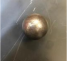
\includegraphics[scale=0.6]{Images/ima1.png}
        \caption{aaaaaaaa}
        \label{fig:ima1}
    \end{figure}
\end{minipage}
\section{Procedimiento}
\begin{minipage}{0.2\linewidth}
    \begin{figure}[H]
        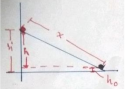
\includegraphics[scale=0.8]{Images/ima2.png}
        \caption{}
        \label{fig:ima2}
    \end{figure}
\end{minipage}
\begin{minipage}{0.6\linewidth}
    Apoyada sobre el soporte universal, se colocó una rampa de
longitud x = 1.83m muescada por el centro e inclinada en
un ángulo variable, por la que se rodó una esfera de radio
R = 1.15cm. Al inicio del plano se colocó la paleta iman-
tada del cronómetro y al final se colocó la paleta detectora.
Como se dijo antes, se varió el ángulo del riel para obtener
\end{minipage}
\begin{minipage}{0.2\linewidth}
    \begin{figure}[H]
        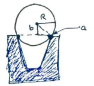
\includegraphics[scale=1]{Images/ima3.png}
        \caption{}
        \label{fig:ima3}
    \end{figure}
\end{minipage}
diferentes tiempos al dejar rodar la esfera. Por razones técnicas, se obtuvo la altura real a través de la que
rodó la esfera restando h 0 de h‘, como se aprecia en el diagrama\\
\begin{minipage}{0.4\linewidth}
    \begin{table}[H]
        \begin{tabular}{|c|c|c|c|} \hline
            t(s) & h(m)& h0(m)& h(m) \\ \hline
1.13& & &\\ \hline
1.21& & &\\ \hline
1.24& & &\\ \hline
1.29& &2.3 &\\ \hline
1.37& & &\\ \hline
1.58& & &\\ \hline
1.80& & &\\ \hline
        \end{tabular}
        \caption{}
    \end{table}
    \begin{equation*}
        a=1586.154115
    \end{equation*}
\end{minipage}